\documentclass{article}%
\usepackage[T1]{fontenc}%
\usepackage[utf8]{inputenc}%
\usepackage{lmodern}%
\usepackage{textcomp}%
\usepackage{lastpage}%
\usepackage{graphicx}%
%
\usepackage{pgfplots}%
\usepackage{tikz}%
\pgfplotsset{compat=1.16}%
\title{Beam Analysis Report}%
\author{PyLaTeX Report Generator}%
\date{\today}%
%
\begin{document}%
\normalsize%
\maketitle%
\tableofcontents%
\newpage%
\section{Introduction}%
\label{sec:Introduction}%
This report presents a comprehensive analysis of beam loading and structural behavior.%


\begin{figure}[h!]%
\centering%
\includegraphics[width=0.8\textwidth]{assets/beam.png}%
\caption{Simply supported beam under loading}%
\end{figure}

%
\newpage%
\section{Load Data}%
\label{sec:LoadData}%
Beam structural analysis data read from Excel file:%
\begin{center}%
\begin{tabular}{|c|c|c|}%
\hline%
\textbf{Position (x)}&\textbf{Shear Force}&\textbf{Bending Moment}\\%
\hline%
0.0&45.0&0.0\\%
\hline%
1.5&36.0&60.75\\%
\hline%
3.0&27.0&108.0\\%
\hline%
4.5&18.0&141.75\\%
\hline%
6.0&9.0&162.0\\%
\hline%
7.5&0.0&168.75\\%
\hline%
9.0&{-}9.0&162.0\\%
\hline%
10.5&{-}18.0&141.75\\%
\hline%
12.0&27.0&108.0\\%
\hline%
13.5&{-}36.0&60.75\\%
\hline%
15.0&{-}45.0&0.0\\%
\hline%
\end{tabular}%
\end{center}

%
\section{Analysis}%
\label{sec:Analysis}%
Shear Force Diagram (SFD) and Bending Moment Diagram (BMD) analysis:%

\begin{center}
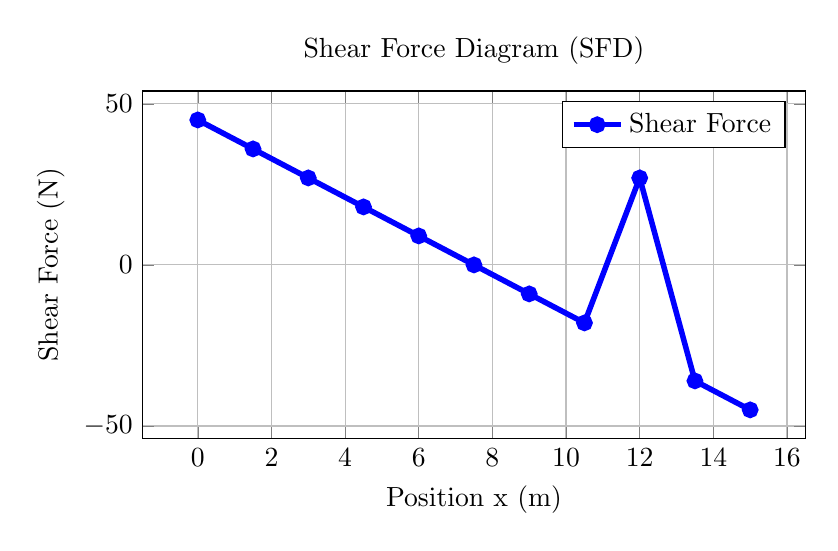
\begin{tikzpicture}
  \begin{axis}[
    title={Shear Force Diagram (SFD)},
    xlabel=Position x (m),
    ylabel=Shear Force (N),
    grid=both,
    width=10cm,
    height=6cm,
    legend pos=north east
  ]
  \addplot[color=blue, mark=*, line width=2pt] coordinates {
    (0.0,45.0) (1.5,36.0) (3.0,27.0) (4.5,18.0) (6.0,9.0) (7.5,0.0) (9.0,-9.0) (10.5,-18.0) (12.0,27.0) (13.5,-36.0) (15.0,-45.0)
  };
  \addlegendentry{Shear Force}
  \end{axis}
\end{tikzpicture}
\end{center}
    %
%

\begin{center}
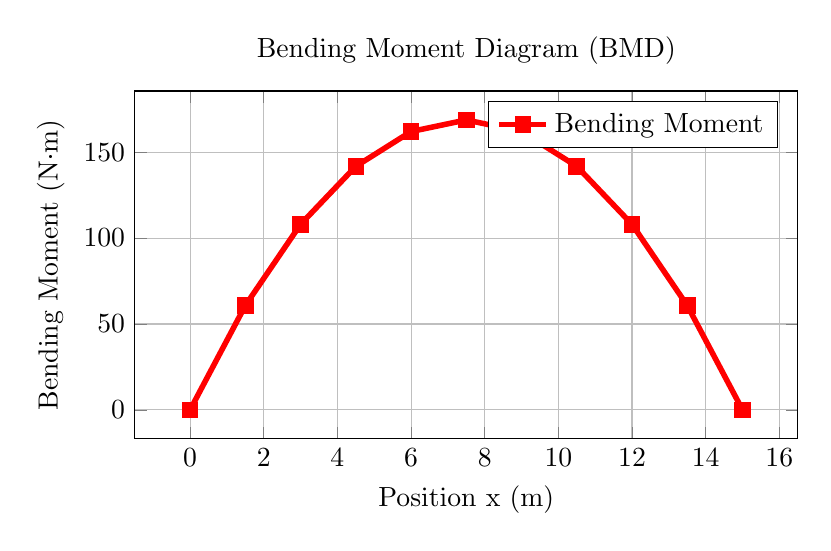
\begin{tikzpicture}
  \begin{axis}[
    title={Bending Moment Diagram (BMD)},
    xlabel=Position x (m),
    ylabel=Bending Moment (N·m),
    grid=both,
    width=10cm,
    height=6cm,
    legend pos=north east
  ]
  \addplot[color=red, mark=square*, line width=2pt] coordinates {
    (0.0,0.00) (1.5,60.75) (3.0,108.00) (4.5,141.75) (6.0,162.00) (7.5,168.75) (9.0,162.00) (10.5,141.75) (12.0,108.00) (13.5,60.75) (15.0,0.00)
  };
  \addlegendentry{Bending Moment}
  \end{axis}
\end{tikzpicture}
\end{center}
    

%
\end{document}